\chapter{Implementation \label{implementation}}

This chapter presents the algorithm for checking composition, the implementation of activations, the implementation of heaps, and the implementation of two schedulers for an interpreter designed for the language presented in chapter~\ref{language}.

\paragraph{Interpreter organization and implementation.}
The interpreter has an orthodox design consisting of a scanner, a parser, a sequence of semantic checks, a code generation phase, composition checks, and an execution phase.
The interpretter is implemented in C++.
Flex and Bison were used to implement the scanner and parser, respectively.
The semantic checks include type checking and checks to support the enforcement of \verb+const+ and \verb+foreign+ intrinsic and dereference mutability.
The implementation of these checks follow the requirements set forth in chapter~\ref{language}.
The code generation phase converts the AST into a tree of stack operations.
The execution phase begins by initializing the instances by calling the initializer associated with each instance.
The scheduler then proceeds by selecting and executing actions with weak fairness.
Scheduler implementations use the POSIX threads (pthreads) library for concurrent execution and synchronization.

\section{Enforcing Sound Composition}

\subsection{Background}

This section outlines the algorithm for checking the composition semantics of reactive components.
As described in chapter~\ref{model}, one of the goals for the reactive component model is to facilitate the construction of complex reactive systems by composition.
The composition semantics of reactive components overcome the limitations of I/O automata and UNITY but introduce concurrency hazards that may result in systems that are not well defined.
The two hazards to be avoided are non-deterministic transactions arising from the same state being updated by multiple transitions within the transaction and recursive transactions arising from cycles in composition.
The goal of the composition check is to determine if a system is free of these hazards.

The check for sound composition is a holistic problem.
Ports facilitate third-party composition by being opaque meaning that the action or reaction activating a port cannot know or care about the state transitions executed as a result of activating the port.
The state involved in a transaction is not known until the components are instantiated and the ports bound.
Thus, the check for sound composition requires a complete understanding of the system.
To this end, the algorithm described in this section leverages the static system assumption.
We leave relaxing the static system assumption, which will require extending the model and proposed check, as future work.

The language semantics of chapter~\ref{model} enforce a number of assumptions that allow the composition check to be formulated as set of simple graph- and set-theoretic problems.
Activation statements are limited to the bodies of actions and reactions and port calls are limited to activation statements.
Activation statements terminate the execution of an action or reaction meaning at most one will be called per action or reaction body.
Thus, a transaction can be viewed as a directed graph where each node is an action or reaction and edges indicate that the source action or reaction activates the target reaction.
With this graph in place, the state involved in a transaction can be deduced by treating the component instances as a proxies for their state variables by creating sets of instances and evaluating the sets for compatibility.

\subsection{Algorithm Sketch}

\paragraph{Enumerate instances and ports.}
The first step to analyzing composition is to enumerate the components in the system.
The top-level components are given by the declared instances.
Sub-components are enumerated by recursively instantiating fields that are also components.
Fields that are ports are also enumerated.

\paragraph{Enumerate bindings.}
Let $I$ be a component instance of type $T$.
Associated with $T$ is a set of binders $B$.
Each binder $b \in B$ is evaluated for $I$ to create a set of bindings.
A binding either binds a push port to a reaction or a getter to a pull port.
The result of enumerating the bindings is two tabular functions.
The function $reactions: (I,Push) \to \{(I,Reaction)\}$ maps an instance/push port pair to a set of instance/reaction pairs.
The function $getter: (I,Pull) \to \{(I,Getter)\}$ maps an instance/pull port pair to a set of instance/getter pairs.

\paragraph{Check bindings.}
Inverting $reactions$ yields a function that maps an instance/reaction pair to a set of instance/push port pairs $reactions^{-1}: (I,Reaction) \to \{(I,Push)\}$.
The $reactions^{-1}$ function is used to ensure that a reaction is bound to one push port or not bound:
\begin{displaymath}
\forall (I,Reaction) : |reactions^{-1} (I,Reaction)| \leq 1
\end{displaymath}
The $getter$ function is used to ensure that a pull port is bound to exactly one getter:
\begin{displaymath}
\forall (I,Pull) : |getters (I,Pull)| = 1
\end{displaymath}

\paragraph{Enumerate transactions.}
Let $I$ be a component instance of type $T$.
Associated with $T$ is a set of actions $A$.
Each action $a \in A$ is evaluated for $I$ to create a transaction.
A \emph{transaction} is a directed graph constructed as follows:
\begin{enumerate}
\item The root is $(I,a)$.
\item The descendants of the root are the activations in $a$.
\item The descendants of the activations are the push ports named in each activation.
\item The descendants of the push ports are the reactions bound to the push ports given by $reactions$.
\item This process is then repeated for each instance/reaction leaf.
\end{enumerate}
Figure~\ref{transaction} shows an example transaction.

\begin{figure}
\centering
%%\resizebox{\textwidth}{!}{%
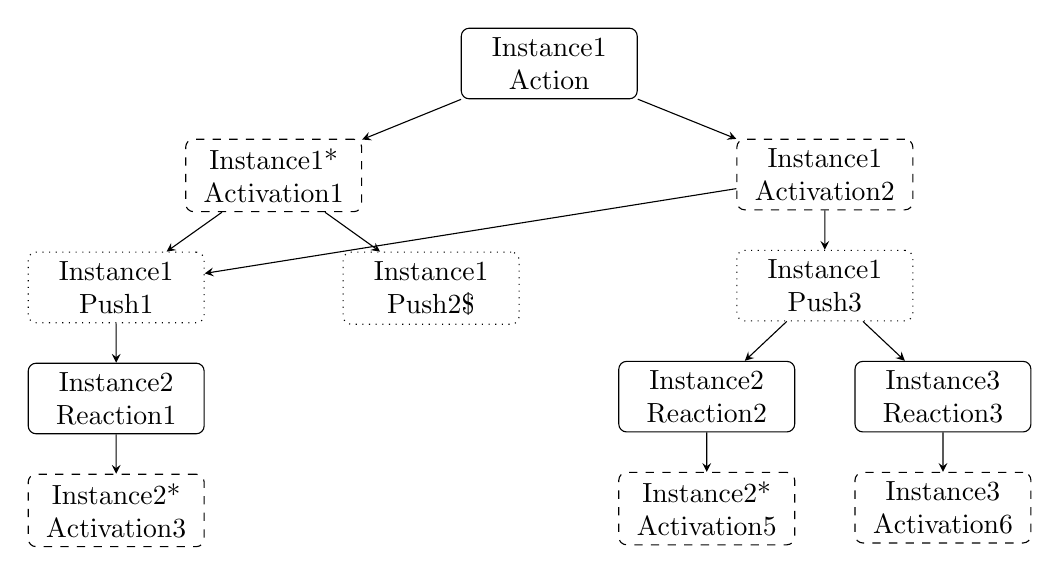
\begin{tikzpicture}[
    arrowstyle/.style={draw, -stealth},
    edge from parent/.style={draw, -stealth},
    reaction/.style={rectangle, draw, rounded corners=1mm, text width=2cm,
        text centered, anchor=north},
    activation/.style={rectangle, draw, rounded corners=1mm, dashed, text width=2cm,
        text centered, anchor=north},
    push/.style={rectangle, draw, rounded corners=1mm, dotted, text width=2cm,
        text centered, anchor=north},
    level 1/.style={sibling distance=7.0cm},
    level 2/.style={sibling distance=4.0cm},
    level 3/.style={sibling distance=3.0cm},
    level distance=0.5cm, growth parent anchor=south
]
\node (Action) [reaction] {Instance1 Action}
  child {
    node (Activation01) [activation] {Instance1* Activation1}
    child {
      node (Push01) [push] {Instance1 Push1}
      child {
        node (Rection01) [reaction] {Instance2 Reaction1}
        child {
          node (Activation03) [activation] {Instance2* Activation3}
        }
      }
    }
    child {
      node (Push02) [push] {Instance1 Push2\textdollar}
    }
  }
  child {
    node (Activation02) [activation] {Instance1 Activation2}
    child {
      node (Push03) [push] {Instance1 Push3}
      child {
        node (Rection02) [reaction] {Instance2 Reaction2}
        child {
          node (Activation04) [activation] {Instance2* Activation5}
        }
      }
      child {
        node (Rection03) [reaction] {Instance3 Reaction3}
        child {
          node (Activation05) [activation] {Instance3 Activation6}
        }
      }
    }
  }
;

\draw[arrowstyle] (Activation02) -- (Push01);

\end{tikzpicture}
%%}%
\caption{Example transaction\label{transaction}}
\end{figure}

\begin{figure}
\centering
%%\resizebox{\textwidth}{!}{%
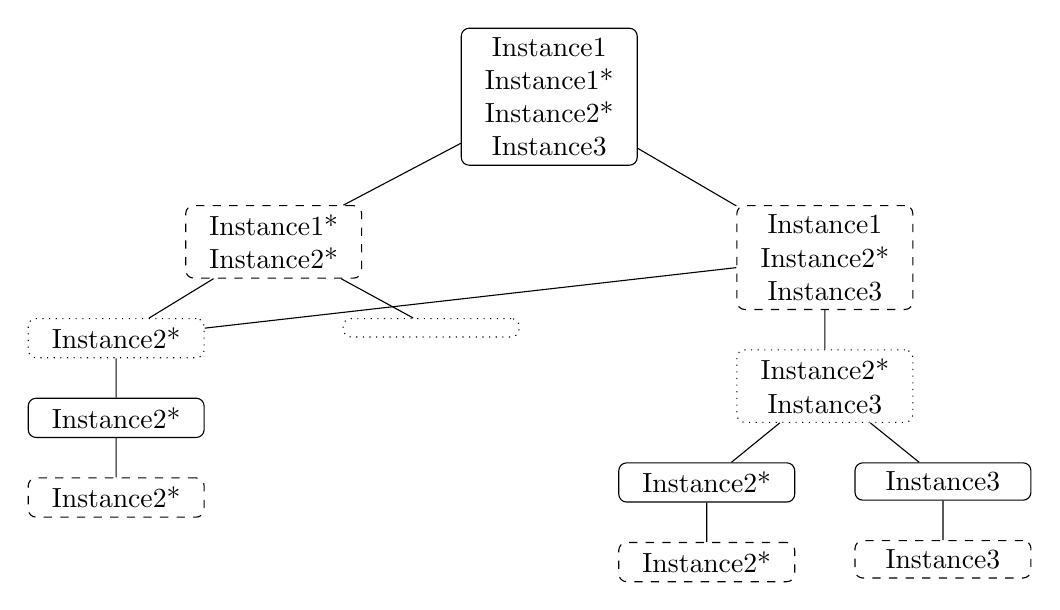
\begin{tikzpicture}[
    reaction/.style={rectangle, draw, rounded corners=1mm, text width=2cm,
        text centered, anchor=north},
    activation/.style={rectangle, draw, rounded corners=1mm, dashed, text width=2cm,
        text centered, anchor=north},
    push/.style={rectangle, draw, rounded corners=1mm, dotted, text width=2cm,
        text centered, anchor=north},
    level 1/.style={sibling distance=7.0cm},
    level 2/.style={sibling distance=4.0cm},
    level 3/.style={sibling distance=3.0cm},
    level distance=0.5cm, growth parent anchor=south
]
\node (Action) [reaction] {Instance1 Instance1* Instance2* Instance3}
  child {
    node (Activation01) [activation] {Instance1* Instance2*}
    child {
      node (Push01) [push] {Instance2*}
      child {
        node (Rection01) [reaction] {Instance2*}
        child {
          node (Activation03) [activation] {Instance2*}
        }
      }
    }
    child {
      node (Push02) [push] {}
    }
  }
  child {
    node (Activation02) [activation] {Instance1 Instance2* Instance3}
    child {
      node (Push03) [push] {Instance2* Instance3}
      child {
        node (Rection02) [reaction] {Instance2*}
        child {
          node (Activation04) [activation] {Instance2*}
        }
      }
      child {
        node (Rection03) [reaction] {Instance3}
        child {
          node (Activation05) [activation] {Instance3}
        }
      }
    }
  }
;

\draw (Activation02) -- (Push01);

\end{tikzpicture}
%%}%
\caption{Example instance set calculation\label{instance_sets}}
\end{figure}

A recursive transaction is formed when a reaction activates itself through the set of bindings or a getter calls itself which appears as a cycle in the transaction graph.
The interpreter contains an implementation of Tarjan's algorithm~\cite{tarjan1976} to detect cycles.

A non-deterministic transaction occurs when the same state is manipulated by multiple transitions.
Thus, the interpreter must determine what state is manipulated in a transaction to determine if the constituent transitions are compatible.
The interpreter uses a component instance as a proxy for its state variables and determines how the state is accessed in each transition.
The possible access patterns include:
\begin{description}
  \item[WRITE] at least one state variable may be mutated (* in figure~\ref{transaction})
  \item[READ] at least one state variable is accessed but no state variables are mutated
  \item[NONE] no state variables are accessed
\end{description}
The current implementation uses a conservative static analysis of the body of an activate statement to determine if the activation mutates the state of the component.
For composition analysis, state variable access need only be determined for the mutable phase.
However, performing a parallel analysis for the immutable phase provides a complete description of state access in a transaction.
State variable access is used by multi-threaded schedulers to determine which transactions can be executed in parallel.

The check for non-deterministic transactions continues by determining that all possible executions of a transaction are deterministic.
This check is performed in two steps.
First, a set of instances/access pairs is computed for each node in the transaction.
If the node is not an activation, then the set of instances is the union of the instances of its children.
If the node is an activation, then the set of instances is the union of the instances of its children and the instance implied by the activation excluding instances with NONE access.
Figure~\ref{instance_sets} shows the instance set calculation for the transaction in figure~\ref{transaction}.
The root shows that Instance1 does not change in at least one activation (Instance1) and may change in at least one activation (Instance1*), that Instance2 may change in every activation (Instance2*), and that Instance3 is read-only in this transaction (Instance3).
The empty node in figure~\ref{instance_sets} comes from an unbound push port.

The second step of the check for non-deterministic transactions is to verify that a mutated instance appears in at most one child node instance set for the activation and push port nodes.
This check succeeds everywhere but Activation2 in figures~\ref{transaction}~and~\ref{instance_sets} as Instance2* appears in both children.
The activation and push port nodes represent activities that will be performed together.
That is, once control passes to an activation statement, all push ports and their bound reactions are activated.
In contrast, activations, as children of action and reaction nodes, represent mutually exclusive alternatives, i.e., at most one activation statement is executed per action/reaction body.
Thus, a mutated instance appearing in two or more children of an activation node or push port node indicates that the state of a component may be mutated in disparate ways leading to a non-deterministic transaction.

\paragraph{Complexity.}
One of the goals of implementing reactive components was to determine if the check for non-determinism has a reasonably efficient implementation.
Maintaining appropriate forward and reverse hash maps of the bindings allow the binding check to be performed in $O(N)$ time where $N$ is the number of ports in the system.
Similarly, the construction of a transaction graph can be performed in $O(|N| + |V|)$ time where $|N|$ is the number of nodes in the transaction and $|V|$ is the number of edges.
Proving that a transaction is acyclic can be performed in $O(|N| + |V|)$ where $|N|$ is the number of nodes and $|V|$ is the number of edges.

A loose upper-bound on the complexity of the instance set calculation for the non-determinism check is $O(k |N|^2 \log (|N|))$ where $|N|$ represents the number of nodes in a transaction and $k$ represents the maximum branching factor in the transaction.
The size of the instance set for the root is $|N|$.
Assuming a naive set implementation, the complexity of computing the instance set for the root is $O(|N| \log (|N|))$.
This must be repeated $k$ times for all nodes in the graph resulting in a final complexity of $O(k |N|^2 \log (|N|))$.

A loose upper-bound on the complexity of the compatibility check for the non-determinism check is also $O(k |N|^2 \log (|N|))$.
Assume that the size of the instance set at each node is $|N|$.
A tree-based set lookup can be performed in $O(\log(|N|))$ time.
The lookup must be performed $k |N|$ times by the parent.
The lookup must repeated for each of the $|N|$ nodes for a combined complexity of $O(k |N|^2 \log (|N|))$.

The complexity of these algorithms has not presented a problem in practice as most of the systems we have implemented have small numbers for $|N|$, $|V|$, and $k$.

\section{Activations}

When executing a transaction, the run-time must execute the immutable phase of all implied state transitions before executing any of the mutable phases.
To accomplish this, the run-time uses a novel calling convention to create a list of deferred contexts and statements that represent the mutable phase of each state transition.
The immutable phase constructs the list and the mutable phase processes the list.
To present the calling convention, we first present some details about the run-time such as the ordinary calling convention and push ports.
We then describe the behavior of the calling convention and illustrate its behavior using an illustrative example.

\paragraph{Ordinary calling convention.}
The ordinary call mechanism in the run-time is based on the C-decl calling convention.
It assumes the existence of an \emph{instruction pointer} which contains the address of the currently executing instruction and a \emph{base pointer} which points to a location in the stack which can be offset to access arguments and local variables.
A ordinary call in the language is accomplished through the following sequence:
\begin{enumerate}
\item (Caller) Push arguments onto the stack, left to right.
\item (Caller) Push the instruction pointer onto the stack and transfer control to the body of the function, method, action, reaction, getter, or initializer.
\item (Callee) Push the base pointer onto the stack and set the base pointer to the top of the stack.
\item (Callee) Reserve space on the stack for local variables.
\item (Callee) Execute the body of the function, method, etc.
\item (Callee) Pop the stack, pop and restore the base pointer, pop and restore the instruction pointer.
\item (Caller) Pop the arguments.
\end{enumerate}
The major difference between this calling convention and C-decl is that the arguments are pushed in the opposite order to match the semantics of Go.
The collection of arguments, previous instruction pointer, previous base pointer, and reserved space is called a \emph{stack frame} or a \emph{call frame}.
Figure~\ref{frame} shows the layout of a normal stack frame.
For this presentation, we assume that the stack grows down, i.e., the previous base pointer has a lower address in memory than the previous instruction pointer.

\begin{figure}
\centering
\resizebox{.5\textwidth}{!}{%
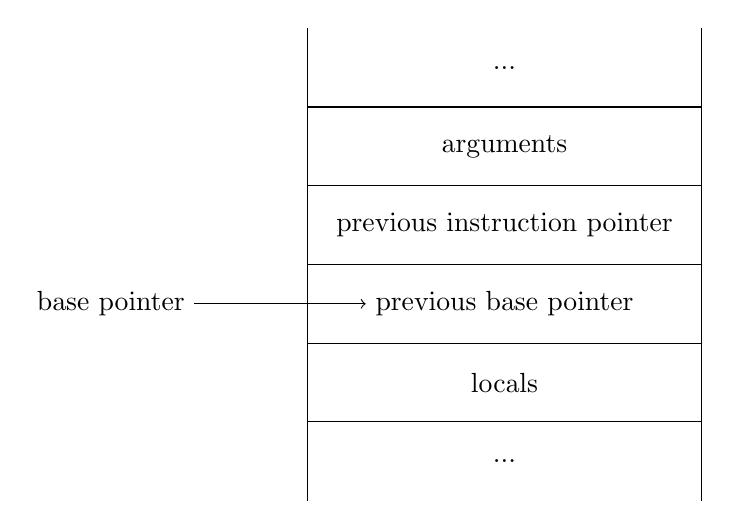
\begin{tikzpicture}
%% component boundary

\draw (0,1) -- (0,7);
\draw (5,1) -- (5,7);

\node at (2.5, 6.5) { ... };
\draw (0,6) -- (5,6);
\node at (2.5, 5.5) { arguments };
\draw (0,5) -- (5,5);
\node at (2.5, 4.5) { previous instruction pointer };
\draw (0,4) -- (5,4);
\node (pbp) at (2.5, 3.5) { previous base pointer };
\draw (0,3) -- (5,3);
\node at (2.5, 2.5) { locals };
\draw (0,2) -- (5,2);
\node at (2.5, 1.5) { ... };

\node (bp) at (-2.5, 3.5) { base pointer };
\draw[->] (bp) -- (pbp);

\end{tikzpicture}
}%
\caption{Diagram of a stack frame\label{frame}.  The stack is depicted as growing down.}
\end{figure}

\paragraph{Push ports.}
A push port is a field in a component.
Physically, a push port is a pointer to a linked list that contains the component pointer/reaction pairs that are bound to the push port.
The run-time populates each push port before execution begins.

\paragraph{Synchronized two-phase calling convention.}
To prepare for the mutable phase, the immutable phase must preserve the stack frame (context) of the action or reaction that executes an activation statement and must record which activation statement was executed so that the same activation can be resumed in the mutable phase.
To accomplish this, we devised the \emph{synchronized two-phase calling convention} which is used to execute activation statements during the immutable phase.

As previously stated, the execution of an activation statement is split into an immutable phase and a mutable phase.
Recall that activation statements may only appear in actions and reactions.
After executing the immutable phase of an activation statement in a reaction, control must be returned to the calling activation statement so that it may activate other push ports.
After executing the immutable phase of an activation statement in an action, control must be returned to the run-time to begin the mutable phase.
In the ordinary calling convention, the call frame for the reaction would be popped, control would be returned to the caller, and the arguments would be popped.
To preserve the call frame for use during the mutable phase, the activation statement returns control to the caller without popping the frame and the caller does not pop the arguments.
Thus, the complete frame for the reaction is preserved on the stack.

Each deferred call frame is added to a list to make it available in the mutable phase.
Let $head$ be a variable containing a pointer, initially nil, which will serve as the head of a linked list.
Before the activation statement returns from the immutable phase, it sets the previous base pointer in the call frame to the value of $head$ and updates head to be the current base pointer which inserts the call frame into the list.
The run-time can iterate over the elements of the list by following the previous base pointer to access all of the call frames that are needed for the mutable phase.
If the list is empty ($head$ is nil), then no activation statement was executed and the mutable phase may be skipped.

The final piece of information that must be recorded is the activation statement or rather the body of the activation statement so that it is accessible in the mutable phase.
Before returning from the immutable phase, the activation statement records the body of the activation statement in the previous instruction pointer slot of the call frame.
It is safe to use the previous instruction pointer because it is not used beyond the immediate return.
Furthermore, it is at a fixed location which allows it to be accessed in any deferred call frame.

The synchronized two-phase calling convention is used when executing an activation statement and proceeds as follows:
\begin{enumerate}
\item Save the previous base pointer of the current stack frame in $bp$.
\item Set the previous base pointer of the current stack frame to the value of $head$.
\item Set $head$ to the value of the base pointer.
\item Save the previous instruction pointer of the current stack frame in $ip$.
\item Set the previous instruction pointer of the current stack frame to the body of the activation statement.
\item For each push port in the port call list:
  \begin{enumerate}
  \item Push the arguments to the push port onto the stack.\label{step1}
  \item For each component pointer/reaction pair in the push port:
    \begin{enumerate}
    \item Push the component pointer onto the stack.
    \item Copy the arguments prepared in~\ref{step1} onto the stack.
    \item Call the reaction.
    \end{enumerate}
  \end{enumerate}
\item Set the base pointer to the value of $bp$ and return control to the value of $ip$.
\end{enumerate}

The synchronized two-phase calling convention evaluates the arguments to a push port once and passes a copy to each bound reaction.
One alternative is to evaluate the arguments for each bound reaction.
This means that the arguments may not be evaluated, i.e., the push port is not bound to any reactions, or may be evaluated multiple times.
If the arguments contain an expression with side-effects, then the behavior of the code becomes dependent on composition.
While this may be desirable in some cases, we opted for making a port call resemble ordinary function call as much as possible.
This sentiment also influenced our decision to pass a copy of the arguments to each reaction as opposed to reusing the same set of prepared arguments.
Since each reaction starts with a copy of the arguments, it is free to manipulate them as allowed by the semantics of Go.
Furthermore, the arguments are available in the mutable phase which obviates the need to make local copies of arguments.
This approach assumes that copying arguments does not generate significant overhead.

%% After an activation statement calls the last push port, it makes temporary copies of the instruction pointer and base pointer of the caller.
%% It may then safely overwrite the base pointer to insert itself into the list of mutable phase call frames and it may safely overwrite the instruction pointer with the body of the activation statement.

The major caveat when using the synchronized two-phase calling convention is that it must be assumed that the stack pointer changes when calling a push port.
To illustrate why this is an issue, consider the case when a caller wishes to preserve the contents of a register.
One strategy is to push the contents of the register onto the stack, perform the call, and then pop the value from the stack into the register.
After calling a push port, the caller may no longer assume that the previous value of the register is at the top of the stack.
The easy work-around is to allocate local variables, i.e., variables whose addresses are relative to the base pointer instead of the stack pointer, for saving temporary values that must persists across a push port call.
In the same way, the variables used to iterate over the list of component/reaction pairs in a push port should be allocated as local variables so that they may survive the calls to the reactions.

\paragraph{The mutable phase.}
The mutable phase consists of executing all of the deferred activation statements.
The algorithm for doing so is as follows:
\begin{enumerate}
\item If the value of $head$ is nil, stop.  Otherwise, set the base pointer to the value in $head$.
\item Transfer control to the instruction indicated by the previous instruction pointer\label{transfer}.  Execution continues until the body of the activation statement implicitly or explicitly returns.
\item If the previous base pointer is nil, stop.  Otherwise, set the base pointer to the previous base pointer and go to \ref{transfer}.
\end{enumerate}

The algorithm iterates over the list of deferred call frames accessible through $head$.
The last element in the list is indicated by a previous base pointer that is nil.
Transfer is controlled to the previous instruction pointer which contains the body of the activation statement.

\begin{figure}
\centering
\resizebox{.75\textwidth}{!}{%
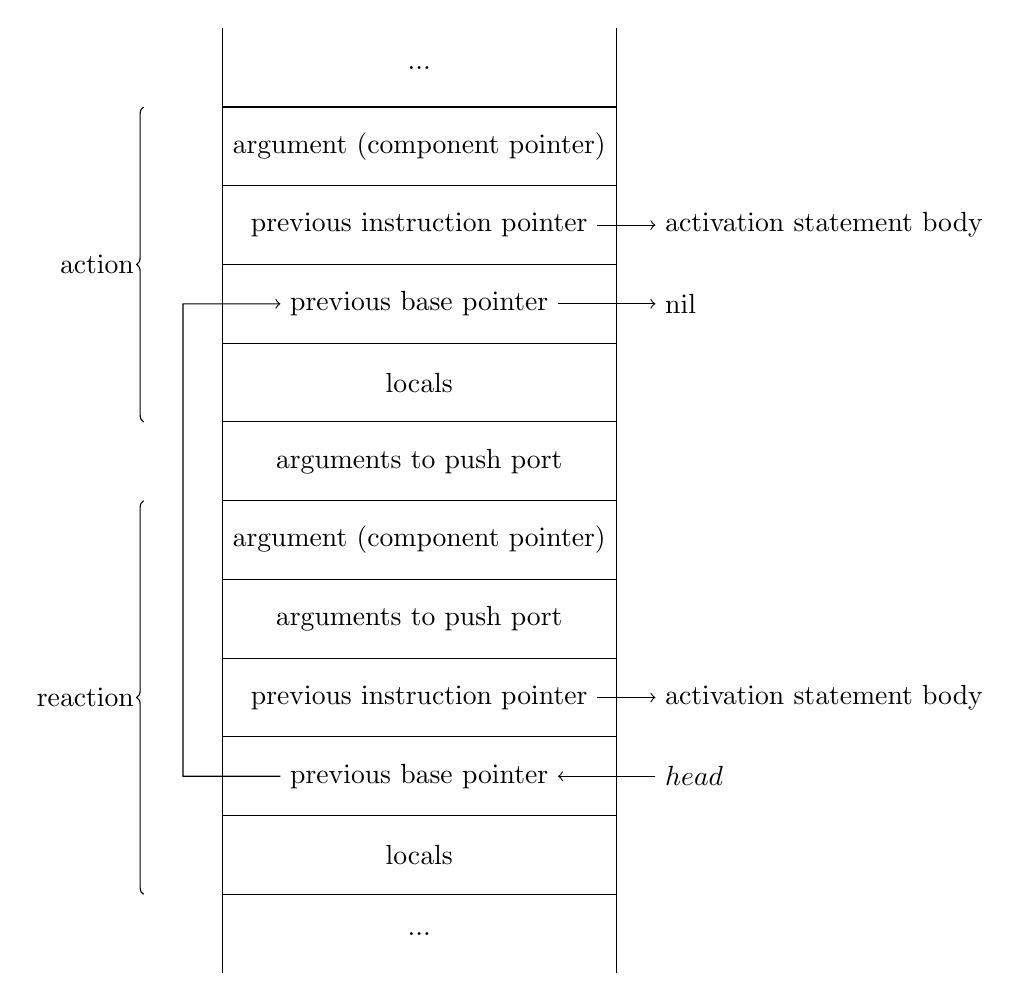
\begin{tikzpicture}
%% component boundary

\draw (0,-5) -- (0,7);
\draw (5,-5) -- (5,7);

\node at (2.5, 6.5) { ... };
\draw (0,6) -- (5,6);
\node at (2.5, 5.5) { argument (component pointer) };
\draw (0,5) -- (5,5);
\node (pip1) at (2.5, 4.5) { previous instruction pointer };
\draw (0,4) -- (5,4);
\node (pbp1) at (2.5, 3.5) { previous base pointer };
\draw (0,3) -- (5,3);
\node at (2.5, 2.5) { locals };
\draw (0,2) -- (5,2);
\node at (2.5, 1.5) { arguments to push port };
\draw (0,1) -- (5,1);
\node at (2.5, .5) { argument (component pointer) };
\draw (0,0) -- (5,0);
\node at (2.5, -.5) { arguments to push port };
\draw (0,-1) -- (5,-1);
\node (pip2) at (2.5, -1.5) { previous instruction pointer };
\draw (0,-2) -- (5,-2);
\node (pbp2) at (2.5, -2.5) { previous base pointer };
\draw (0,-3) -- (5,-3);
\node at (2.5, -3.5) { locals };
\draw (0,-4) -- (5,-4);
\node at (2.5, -4.5) { ... };

\node[anchor=west] (as1) at (5.5, 4.5) { activation statement body };
\draw[->] (pip1) -- (as1);
\node[anchor=west] (as2) at (5.5, -1.5) { activation statement body };
\draw[->] (pip2) -- (as2);

\draw[->] (pbp2) -- ++(-3,0) -- ++(0,6) -- (pbp1);

\node[anchor=west] (nil) at (5.5, 3.5) { nil };
\draw[->] (pbp1) -- (nil);

\node[anchor=west] (head) at (5.5, -2.5) { $head$ };
\draw[->] (head) -- (pbp2);

\draw[decorate,decoration={brace}] (-1,2) -- (-1,6) node[anchor=east,midway] { action };

\draw[decorate,decoration={brace}] (-1,-4) -- (-1,1) node[anchor=east,midway] { reaction };

\end{tikzpicture}
}%
\caption{Diagram of the stack after the immutable phase when an action activates a single reaction.\label{activation_ex_1}}
\end{figure}

\paragraph{Example:  one action, one reaction.}
Suppose an action activates a single push port that is bound to a single reaction and the reaction has a single activation that does not activate any push ports.
Figure~\ref{activation_ex_1} shows a diagram of the stack after the immutable phase for this scenario.
The stack contains two frames, one corresponding to the action and one corresponding to the reaction.
The $head$ variable points to the reaction frame which in turn points to the action frame using the previous base pointer slot.
The action frame points to nil indicating that it is the last frame in the list.
The previous instruction pointers point to the bodies of the activation statements.
Between the frames are the push port arguments which are duplicated for the call to the reaction.
If the push port had been bound to multiple reactions, then the reaction portion of the diagram would be replicated to match the number of bound reactions.
If multiple push ports were activated by the activation statement, then additional push port arguments and reactions would appear on the stack.

\paragraph{Calling convention efficiency.}
The synchronized two-phase calling convention has the potential to be as efficient as function call and method call.
The proposed calling convention can be implemented directly on modern hardware.
Popular modern architectures like x86 and x86\_64 contain all of the registers and instructions necessary to support the synchronized two-phase calling convention.
The synchronized two-phase calling convention relies solely on the stack which means that the underlying operating system must setup the stack, back it with memory pages, etc.
More importantly, it avoids the overhead of heap allocation.
Port calls resemble virtual method calls in that the reactions must be looked up before they can be executed.
However, this lookup could be avoided by inlining the body of each reaction using the substitutional equivalence property.
This could be performed prior to execution or during execution using just-in-time compilation techniques.

\section{Heaps}

In this section, we describe the implementation of the heap data type introduced in chapter~\ref{language} and our approach to garbage collection.
Our approach to implementing dynamic memory allocation and garbage collection was shaped by the independence of state required by the semantics of reactive components.
Thus, instead of relying on a single global heap, the implementation contains a heap for each component that can be garbage collected independently of the others.
This independence allows garbage collection to be performed concurrently with other activities using simple, single-threaded algorithms.

\paragraph{Slots and blocks.}
A \emph{slot} is the smallest unit of memory that can be dynamically allocated.
Typically, a slot is the size of two pointers.
A \emph{block} is an extent of memory and a set of bits indicating the allocation status of each slot in the extent.
The status bits indicate if a slot is allocated, if a slot is the beginning of an object, and if the slot has been marked by the mark-and-sweep algorithm.
Blocks also contain left and right pointers that allow them to be formed into a binary tree sorted by the address of the extent.

\paragraph{Mark-and-sweep garbage collection.}
We implemented a simple mark-and-sweep algorithm to collect garbage in a tree of blocks.
The core of the marking phase involves scanning extents for pointers to objects.
When the algorithm comes across a slot that is allocated, marked, and which contains a pointer that points to a location in the tree of blocks, it marks the object indicated by the pointer which must also be allocated.
The algorithm is bootstrapped by marking all slots in a designated root object.
The algorithm repeatedly scans the extents in the tree of blocks until no new marks can be added.
At this point, the sweep phase resets the allocated bit for all slots that are allocated but not marked and resets the marked bit for the next run of the algorithm.
A block that is not marked, meaning that none of its slots were marked, is removed from the tree of blocks and deallocated.

\paragraph{Heaps.}
A \emph{heap} contains a root block, a list of unallocated chunks of memory (free list), and pointers to create a tree structure.
When allocating an object from a heap, the heap attempts to find an adequate chunk using the free list using a first-fit policy.
If this fails, the heap allocates a new block, inserts it into the tree and free list, and then allocates again using the newly inserted chunk.
The sweep phase of the mark-and-sweep algorithm reconstructs the free list.

As described in chapter~\ref{language}, every component has an associated heap.
A heap of this kind is called an \emph{implicit heap}.
Heaps that are created via \verb+new+ and passed to \verb+move+, \verb+merge+, and \verb+change+ are called \emph{explicit heaps}.
All heaps have a distinguished root object.
The marking phase of the mark-and-sweep algorithm is seeded with this root object.
The root object of an implicit heap is the static component state of the component that owns the heap.
The root object of an explicit heap is an object that is allocated in the same heap.

The semantics of reactive components allow heaps to form strict hierarchies, i.e., a tree structure where the root of the tree is an implicit heap and the internal nodes and leaves of the tree are explicit heaps.
A strict hierarchy gives a graphical interpretation to merge and move operations.
A move operation moves a sub-tree from one location to another location.
 Merging a heap $h$ into another heap $p$ involves removing $h$ from the tree, inserting the blocks of $h$ into the tree of blocks of $p$, merging the free list of $h$ into the free list of $p$, and inserting the children of $h$ as children of $p$.

\paragraph{The active heap.}
Logically, the run-time maintains a stack of heaps where the top of the stack represents the \emph{active heap}.
The active heap is used to satisfy all dynamic memory requests, e.g., calls to \verb+new+.
The implicit heap that is associated with the receiving component is pushed/popped upon entering/leaving an action, reaction, getter, or initializer.
\verb+change+ statements are used to push and pop explicit heaps.
Thus, the call stack, specifically, the change statements that are active on the call stack, implement the stack of heaps.
When a new heap is created, it is inserted as a child of the active heap.

\paragraph{Atomicity.}
Chapter~\ref{language} describes how the semantics of reactive components permit concurrent access to heaps.
The first scenario where this may occur is when a heap is passed to a push port that is bound to multiple reactions.
The semantics of reactive components allow the reactions to be executed concurrently.
Thus, two different threads may be attempt to move/merge the same heap at the same time.
The second scenario occurs when a component is concurrently accessed in multiple transactions that don't mutate the state of the component.
The action, reaction, or getter is allowed to allocate memory which means that heaps must correctly handle concurrent access.
Our implementation of heaps uses the Thread Safe Interface pattern~\cite{schmidt2000pattern} to synchronize access to heaps when allocating, moving, and merging.

\paragraph{Heap links.}
Heaps are exposed to users via pointers to heaps, e.g., \verb+*heap int+.
These pointers to heaps can be stored in objects allocated in another heap.
The semantics of \verb+change+, \verb+merge+, and \verb+move+ ensure that the parent-child relationships formed by pointers to heaps match exactly those known by the run-time system.
The two rules that enforce this behavior are 1) \verb+merge+ and \verb+move+ fail for any heap that is already on the stack of active heaps and 2) all pointers in scope become foreign in the body of a change statement.
The second rule forces the user to \verb+move+ heaps if they desire to change the hierarchy because pointers with foreign dereference mutability cannot be stored.
Recall that the stack of active heaps is setup by active \verb+change+ statements.
Using the inductive argument that the parent-child relationship was previously correct, then the ancestors of the active heap must all appear in the stack of active heaps.
Thus, failing to \verb+merge+ and \verb+move+ heaps on the active stack prevents the formation of cycles.

\begin{figure}
\centering
%%\resizebox{\textwidth}{!}{%
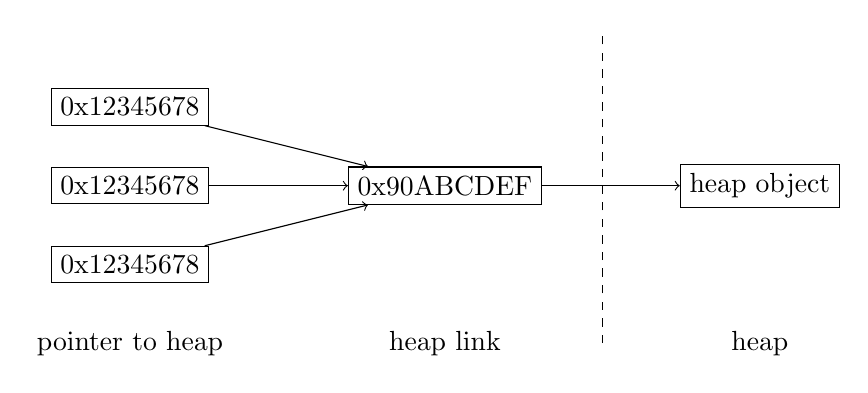
\begin{tikzpicture}
\node [rectangle, draw] (p1) at (0,1) {0x12345678};
\node [rectangle, draw] (p2) at (0,0) {0x12345678};
\node [rectangle, draw] (p3) at (0,-1) {0x12345678};
\node at (0,-2) {pointer to heap};
\node [rectangle, draw] (hl) at (4,0) {0x90ABCDEF};
\node at (4,-2) {heap link};
\node [rectangle, draw] (heap) at (8,0) {heap object};
\node at (8,-2) {heap};
\draw [->] (p1) -- (hl);
\draw [->] (p2) -- (hl);
\draw [->] (p3) -- (hl);
\draw [->] (hl) -- (heap);
\draw [dashed] (6, -2) -- (6, 2);
\end{tikzpicture}
%%}%
\cprotect\caption{Example illustrating heap links\label{heap_link}.  The objects on the far left represent user-level pointers to heaps, e.g., \verb+* heap int+.  The middle object is a heap link which contains the address of the child heap which appears on the far right.}
\end{figure}

As illustrated in figure~\ref{heap_link}, a user-level pointer to a heap points to an object called a heap link which in turn points to a heap.
The objects on the left side of the diagram are objects in the parent heap and the object on the right is the child heap.
The extra level of indirection introduced by the heap link concentrates all references to the child heap into one location.
Moving a heap involves reading the pointer out of the heap link and replacing it with \verb+nil+.
This makes the heap inaccessible to the previous owner, i.e., parent, which maintains the isolation of state between reactive components.
The marking phase of the mark-and-sweep algorithm is aware of heap links and marks heaps as being reachable from another heap.
Unreachable heaps are pruned from the hierarchy during garbage collection.

\paragraph{Embarrassingly parallel garbage collection.}
Two features of reactive components permit concurrent garbage collection.
First, the state of each reactive component is isolated which allows garbage collection to be performed on different components at the same time without conflict.
Second, garbage collection can be framed as an action to be executed by the scheduler.
Thus, associated with each component is an action that invokes the garbage collector on the implicit and explicit heaps of the corresponding component.
Furthermore, the action is considered to modify the state of the component which prevents all transactions involving the component from executing concurrently with the garbage collection action.
We assume that the scheduler selects the garbage collection action often enough that no additional invocations of the garbage collector are necessary.
More plainly, we do not trigger the garbage collector in the allocation routine which is the approach taken by most systems using garbage collection.
Most garbage collection algorithms scan the call stack to determine the root objects in the heap.
In our approach, such scanning is useless since the call stack is empty when executing the garbage collection action and the root object is embedded in the implicit heap that is being collected.

\section{Scheduler}

A scheduler is responsible for selecting and executing transactions according to the weak fairness criteria set forth in chapter~\ref{model}.
Of interest to us is the design and implementation of general-purpose multi-threaded schedulers that are capable of executing actions in parallel.
The main inputs to a scheduler are the instances $I$ and transactions $A$ enumerated by the composition analysis.
The instance sets calculated for each transaction are used in multi-threaded schedulers to avoid non-deterministic state transitions.
We introduce some the issues when designing and implementing a scheduler for reactive components through a series of increasingly complex scheduler designs.
The two concrete implementations described later will draw upon the designs of these schedulers.

\subsection{Scheduler Design}

\paragraph{Scheduler criteria.}
A scheduler is \emph{fair} if it meets the weak-fairness criteria set forth in chapter~\ref{model}.
A scheduler is \emph{safe} if it avoids conditions where one transaction is changing the state of the component while another transaction is reading or writing the same state.
A scheduler is \emph{responsible} if it only terminates when the precondition for every action is false.
Obviously, we are interested in fair, safe, and responsible schedulers as these schedulers enforce the semantics of reactive components.
The final criteria for a scheduler is efficiency which typically refers to either the computational complexity or storage complexity associated with its operation.
Of primary interest is the \emph{selection efficiency} or the amount of computation required for the scheduler to determine the next action to execute.

\paragraph{Single-threaded round-robin scheduler.}
Perhaps the simplest scheduler that can be implemented is a single-threaded round-robin scheduler.
This design may be appropriate in the context of uniprocessor embedded systems with tight resource constraints.
The scheduler repeatedly cycles through the list of transactions, evaluating the precondition of each action and executing the body if the precondition was true.
If no action is executed in a cycle, then the scheduler terminates.
This scheduling algorithm is fair by virtue of the strict round-robin policy, safe from the fact that it is single-threaded, and responsible by definition.
The selection efficiency of this algorithm is $O(|A|)$ as illustrated by a system where one action that is perpetually enabled while all of the other actions are perpetually disabled.

\paragraph{Single-threaded scheduler with an action work queue.}
The perceived weakness of the single-threaded round-robin scheduler is the overhead of evaluating preconditions that evaluate to false.
So, instead of cycling through the list of actions, this scheduler maintains a work queue of actions whose preconditions are true.
At initialization time, the scheduler populates the queue by evaluating the precondition for all actions in the system.
The scheduler then repeatedly takes an action from the queue, executes it, and then inserts any newly enabled actions.
To find newly enabled actions, the scheduler uses the instance set generated during composition analysis.
That is, after executing an action, the scheduler tests all of the actions for the components in the instance set and adds them to the queue if necessary.
The scheduler terminates when the work queue is empty.
This scheduling algorithm is fair if the work queue is processed in first-in first-out (FIFO) order, safe because the algorithm is single-threaded, and responsible since an empty work queue implies no action is enabled.

The pathological scenario of the single-threaded round-robin scheduler applies to this scheduler as well so the worst-case selection efficiency of the algorithm is $O(|A|)$.
Assume that the most complex transaction in the system involves $c$ components and some component has a system maximum action count of $a$.
In the worst case, the scheduler must execute $c \times a$ preconditions for every action that it executes.
Thus, the overhead associated with this scheduler is related to the compositional structure of the system which it is executing.
This overhead may be acceptable for systems where $c$ and $a$ are small or for systems whose average work queue size is small compared to the total number of actions in the system.
This suggests that the average number of enabled actions compared to the total number of actions may be useful way to analyze systems and schedulers.
For example, the single-threaded round-robin scheduler would be appropriate for a \emph{heavily enabled} system while the single-threaded scheduler with an action work queue would be appropriate for a \emph{lightly enabled} system.

\paragraph{Single-threaded scheduler with an instance work queue.}
This scheduling algorithm attempts to squeeze a little more performance from the single-threaded scheduler with an action work queue.
This significant difference is that after the scheduler executes an action, it places the component instances that might have changed state into the work queue.
The work queue is initialized with all of the components in the system.
When processing a component on the work queue, the scheduler cycles through all of the actions for that particular component.
The increase in performance comes from deferring the evaluations of the preconditions until absolutely necessary.
The behavior on which this scheduler attempts to capitalize is components that are rarely involved in transactions.
An instance is \emph{enabled} if at least one of its actions is enabled.
Thus, this scheduler is appropriate for systems that are lightly enabled from the instance perspective.

\paragraph{Multi-threaded global round-robin scheduler.}
This scheduler runs $P > 1$ copies of a round-robin scheduler in parallel.
To be safe, we must devise a protocol that allows the threads to avoid concurrently executing actions that may mutate the same state.
Using the assumption that a component instance is a proxy for its state variables, the scheduler locks all instances in the instance set before evaluating the precondition and executing the action.
Recall that composition analysis determines the set of components that are involved in a transaction and how they are accessed (WRITE, READ, or NONE).
The acquired lock corresponds to the access type which allows multiple threads to be reading a component but only one thread to be writing.
The locks are acquired in a determined order to avoid deadlock (Havender's Principle).
The global mutli-threaded roud-robin scheduler is fair so long as the underlying locking mechanism is fair, i.e., there is no reader or writer starvation.
The algorithm is also responsible as each thread proves to itself that there are no enabled actions left in the system.

The obvious feature of this algorithm is the locking required to coordinate access to component instances.
One negative characteristic caused by the locking is that processors may become idle while waiting for a lock.
Thus, we might look for alternatives that allow a processor to do useful work while waiting for a lock.
Another goal might be to look for ways to coordinate access to component instances without using locks at all.
Chapter~\ref{future_work} describes some ideas toward these goals.

\paragraph{Multi-threaded partitioned round-robin scheduler.}
Rather than have each thread process the entire list of transactions, the multi-threaded partitioned round-robin scheduler divides the list of transactions among the available threads.
Like the global version, this algorithm is fair if the underlying locking mechanism is fair.
Similarly, this algorithm is safe as locks are used to coordinate access to component state.
However, for this algorithm to be responsible, we must add a protocol that allows the threads to detect that the system has reached the termination condition.

The termination protocol consists of a barrier synchronization and then a check to establish the termination condition.
The termination protocol begins when a scheduler thread sends a termination request to the \emph{manager thread}.
To process a termination request, the manager thread stops each scheduler thread and then checks that all transactions are disabled.
If all of the transactions are disabled, the system terminates.
Otherwise, the manager thread restarts the scheduler threads.
A scheduler thread may choose to request termination at any time and different heuristics may be used to determine when a scheduler thread makes the termination request.
Deferring the request has the advantage of avoiding the termination protocol overhead.
For example, a scheduler thread might wait until it makes a complete pass through its list of transactions without executing one before making the request.

The proposed termination protocol is rather disruptive as it must stop the system to check for termination.
Thus, one goal may be to let a thread idle itself and be woken up by active neighbors.
Similarly, the scheduler threads can check for the termination condition in parallel and wake up all of their neighbors if an action is enabled.
Finally, the manager thread may be done away with entirely and the protocol be rewritten as a distributed protocol.

\subsection{Scheduler Implementation}

\paragraph{Multi-threaded scheduler with a global instance work queue.}
The first scheduler that we implemented was a multi-threaded scheduler with a global instance work queue.
The work queue is initialized to contain all of the instances in the system.
The scheduler threads take an instance from the work queue, select and execute all actions in the instance, and insert any instances that might have changed state back into the work queue.
Fairness is achieved by processing the queue in LIFO order and safety is achieved through the aforementioned locking scheme.
The termination protocol for this scheduler involves counting the number of instances that are currently in the queue and the number of instances currently being processed by the scheduler threads.
When this count drops to zero, there are no enabled instances in the system and the system may terminate responsibly.

One potential weakness of this scheduler is that it is based on a global work queue.
The synchronization required to coordinate access to the queue adds a communication overhead and may create contention if the scheduler threads are lightly loaded, i.e., they frequently return to the queue looking for work.
Thus, the scalability of this scheduler is a concern.

\paragraph{Multi-threaded partitioned round-robin scheduler with asynchronous locking and distributed termination.}
One of the goals when designing this scheduler was to avoid the system call overhead of locking observed with the multi-threaded scheduler with a global instance work queue.
The reader/writer locks used to protect each component instance were replaced by asynchronous read/writer locks implemented in user-space.
The asynchronous locks consist of a spin lock, variables indicating the status of the lock, and a queue of requests.
To acquire a lock for a component, a scheduler thread first acquires the spin lock and then checks if the lock can be acquired immediately.
The lock can be acquired immediately if 1) the lock has no owner or 2) the thread is a reader, i.e., it is requesting a read lock, the lock has already been locked by another reader, and there are no writers in the queue.
Otherwise, the request is placed on the queue.
A scheduler thread failing to acquire the lock can either idle itself or attempt to execute a different action.
When a lock is unlocked, the thread at the front of the queue is notified so it may resume processing the action that it was attempting to execute.
The protocol avoids reader and writer starvation and ensures fairness since the queue is processed in LIFO order.

The aforementioned centralized termination protocol has the potential to be disruptive.
Thus, the motivation for a distributed termination protocol is to keep the scheduler threads as busy as possible meaning that the termination protocol is started infrequently and the termination protocol itself aborts as early as possible if the termination condition has not been reached.
For this scheduler, the threads are arranged in a ring and communicate using asynchronous message queues.
Messages are stamped with the id of the originating thread.
Some parts of the protocol forward messages around the ring so a thread receiving a message from itself knows that all of the threads have processed that message.

Like the centralized version, the ring-based distributed termination protocol consists of a synchronization phase and checking phase.
Scheduler threads begin in the RUN state where they are actively cycling through their list of actions.
When a scheduler thread determines that termination may be possible, it sends a message to its neighbor indicating that it is entering the SYNC state.
If the neighbor thread is in the RUN state, it resolves to send a reset message the next time it executes an action which means that the termination condition has not been established.
Otherwise, the neighbor thread itself is already in the SYNC state and forwards the message.
Reset messages are unconditionally forwarded around the ring and cause all threads to enter the RUN state.
Synchronization messages are only forwarded if the thread receiving the message is in the SYNC state.
Thus, if a thread receives its own synchronization message, all other threads in the scheduler are in the SYNC state.
Multiple threads may receive their own synchronization message at the same time.

The goal of the synchronization phase is to establish a common point of reference for determining if any action is enabled.
When a thread receives its own synchronization message, it sends a message to its neighbor that it is entering the CHECK state.
This message is forwarded around the ring causing all of the threads to enter the CHECK state.
The CHECK state is like the modified RUN state in that any executed action causes a reset message to circulate around the ring.
A thread that cycles through its list of actions and finds no enabled actions sends a wait message to its neighbor and enters the WAIT state.
If the neighbor is in the WAIT state, it forwards the message.
If a thread receives its own wait message, then all of the threads are in the WAIT state and the termination condition has been established.
Upon receiving its own wait message, a thread sends a termination message causing all threads to terminate.

\subsection{Scheduler Evaluation}

The utility of the reactive component model rests on the ability to effectively execute reactive programs.
The challenge, then, is to design and implement effective schedulers subject to the constraints and limitations imposed by the model.
The exercise of developing and evaluating schedulers may suggest possible improvements to the model or provide evidence that core features of the model resist efficient implementation.
The definition of an effective scheduler will vary by platform and problem domain.
For example, embedded systems may prefer a single-threaded scheduler with minimal memory requirements and power-awareness.
Our focus in this work is to make progress on a general purpose multi-threaded scheduler.

We propose the following standard queueing metrics for the evaluation of a general-purpose scheduler:
\begin{description}
\item[Throughput] the number of actions executed per second.
\item[Latency] the amount of time between an action becoming enabled and being executed.
\item[Utilization] the fraction of the CPU used.
\end{description}
Given the same system, a scheduler with higher throughput is preferable to a system with lower throughput as it is accomplishing more work per unit time.
The goal in measuring the latency between an action becoming enabled and its execution is to quantify the responsiveness of the scheduler.
Both throughput and latency may be considered for individual actions or aggregated over all actions in the system.
Utilization is a measure of how efficiently the scheduler is using the CPUs and can be used to qualify an improvement in throughput or latency.
For example, a 10\% increase in throughput accompanied by a 10\% increase in utilization is acceptable while a 10\% increase in throughput with a 100\% increase in utilization is not acceptable.

\begin{figure}
\centering
\resizebox{.5\textwidth}{!}{%
\begin{tikzpicture}

\node[draw, ellipse] (Request) at (0,0) {Request};
\node[draw, ellipse] (Response) at (3,0) {Response};
\node[draw, ellipse] (Tick) at (1.5,-1) {Tick};

\draw (Request) -- (Response);
\draw (Tick) -- (Response);

\end{tikzpicture}
}%
\caption{Mutex graph for the clock system.  Each node is a transaction.  Nodes sharing an edge cannot be executed concurrently due to shared state. \label{clock_system_mutex}}
\end{figure}

We used the fully-factored clock system of chapter~\ref{model} to evaluate the two scheduler implementations.
In this system, there are three components of interest which we will designate the Client, the Server, and the Counter.
This system has three transactions:
\begin{itemize}
  \item Request - The client requests the time from the server.  This involves the Client and the Server.
  \item Response - The server responds with the time.  This involves the Client, the Server, and the Counter.
  \item Tick - The counter increments the current time.  This involves the Counter.
\end{itemize}
Figure~\ref{clock_system_mutex} shows the \emph{mutex graph} for the clock system.
Each node in the graph is a transaction.
Nodes sharing an edge cannot be executed concurrently due to shared state.
Conversely, nodes that are not linked by an edge can be executed concurrently.
For the purpose of evaluating schedulers, the clock system has the important characteristic that Request and Tick can be executed concurrently while Response must be executed independently.
Another useful feature of this system is that each component has exactly one action, thus, a  work queue of instances may also be viewed as a work queue of actions.

For comparison, we implemented the clock system using the POSIX threads library (pthreads).
To preserve the spirit of the original design, the custom implementation uses three threads corresponding to the Request, Response, and Tick transactions.
The Request and Response threads share a flag variable that is protected by a mutex and condition variable to implement the asynchronous request/response protocol.
The Response and Tick threads share a counter variable that is protected by a mutex.
For convenience, the custom clock implementation will be called the \emph{clock scheduler}, the multi-threaded scheduler with a global instance work queue will be called will be called the \emph{instance scheduler}, and the multi-threaded partitioned  round-robin scheduler with asynchronous locking and distributed termination will be called the \emph{partitioned scheduler}.
Table~\ref{environment} lists the environment used to perform the scheduler experiments.

\begin{table}
\center
\begin{tabular}{rl}
Machine Model:    & Lenovo G570 Laptop \\
Operating System: & Ubuntu 14.04 \\
Processor:        & Intel Pentium B960 2.20GHz \\
Architecture:     & 64-bit \\
Cores:            & 2 \\
Memory:           & 4GB \\
Kernel:           & 3.13.0-76-generic \#120-Ubuntu SMP \\
Compiler:         & g++ 4.8.4 \\
C library:        & glibc 2.19 \\
POSIX threads:    & glibc 2.19 \\
C++ library:      & glibc++ 3.4.19 \\
\end{tabular}
\caption{Experimental environment used for scheduler testing.\label{environment}}
\end{table}

\begin{figure}
\center
\includegraphics[width=\textwidth]{clock_throughput_cdf.png}
\caption{Cumulative distribution function for the throughput of the clock scheduler. \label{clock_throughput}}
\end{figure}

\begin{figure}
\center
\includegraphics[width=\textwidth]{instance_throughput_cdf.png}
\caption{Cumulative distribution function for the throughput of the instance scheduler. \label{instance_throughput}}
\end{figure}

\begin{figure}
\center
\includegraphics[width=\textwidth]{partitioned_throughput_cdf.png}
\caption{Cumulative distribution function for the throughput of the partitioned scheduler. \label{partitioned_throughput}}
\end{figure}

The throughput of each scheduler was determined by executing the clock system for approximately 10 seconds and counting the number of executed transactions to compute the throughput.
The number of transactions was determined from the program output and does not include the garbage collection actions.
For the instance and partitioned schedulers, the 10 seconds includes parsing the source file, performing the semantic checks, etc.
However, it is long enough to establish a steady state.
The experiment was repeated 1,000 times.
The cumulative distribution function for the throughput of each scheduler is shown in figures~\ref{clock_throughput}, \ref{instance_throughput} and~\ref{partitioned_throughput}.
Based on the shape of distributions, we select the median as the metric for comparison.

The graphs show that the partitioned scheduler achieves a higher average throughput for the clock system.
The average throughput for the instance scheduler was 481340.3 transactions/s while the average throughput for the partitioned scheduler was 496106.7 transactions/s; an increase of 3\%.

Figure~\ref{partitioned_throughput} shows that the partitioned scheduler is bi-modal for the clock system.
The partitioned scheduler randomly and statically allocates transactions to scheduler threads.
This results in four equally possible allocations with two kinds of behavior.
The first allocation is when all transactions are allocated to one thread.
The second allocation is when Request and Tick are allocated to one thread while Response is allocated to the other.
In both of these allocations, the potential concurrency between Request and Tick cannot be exploited.
The third allocation is when Request and Response are allocate to one thread while Tick is allocated to the other.
The fourth allocation is when Response and Tick are allocated to one thread while Request is allocated to the other.
In both of these allocations, the potential concurrency between Request and Tick can be exploited.
Thus, one mode represents configurations where the scheduler is able to take advantage of the potential concurrency in the system leading to higher throughput while the other mode represents configurations where the scheduler is unable to take advantage of the potential concurrency in the system.

\begin{figure}
\center
\includegraphics[width=\textwidth]{instance_throughput_utilization.png}
\caption{Throughput vs. utilization for the instance scheduler. \label{instance_throughput_utilization}}
\end{figure}

\begin{figure}
\center
\includegraphics[width=\textwidth]{partitioned_throughput_utilization.png}
\caption{Throughput vs. utilization for the partitioned scheduler. \label{partitioned_throughput_utilization}}
\end{figure}

Figures~\ref{instance_throughput_utilization} and~\ref{partitioned_throughput_utilization} show plots of utilization against throughput for the instance and partitioned scheduler.
The utilization was calculated as the ratio of the total CPU time (user and system) to the wall clock time.
The utilization includes the time spent executing transactions, scheduler overhead, system call overhead, and overhead for the garbage collection actions.
The maximum utilization for this experiments is 2.0 since the system contains 2 CPUs.
The average utilization for the instance scheduler was 1.497 and the average utilization for the partitioned scheduler was 1.718; an increase of 15\%.
Thus, the question is whether or not a 3\% increase in throughput is worth a 15\% increase in utilization?
Alternatively, we may attempt to reduce the utilization caused by the scheduler through more efficient selection.

\begin{figure}
\center
\includegraphics[width=\textwidth]{instance_latency_cdf.png}
\caption{Cumulative distribution function for the latency of the instance scheduler. \label{instance_latency}}
\end{figure}

\begin{figure}
\center
\includegraphics[width=\textwidth]{partitioned_latency_cdf.png}
\caption{Cumulative distribution function for the latency of the partitioned scheduler. \label{partitioned_latency}}
\end{figure}

The latency of each scheduler was determined by executing the clock system for approximately 10 seconds and measuring the elapsed time between the transaction becoming enabled and being executed.
In the clock system, Request enables Response, Response enables Request, and Tick is always enabled.
Thus, it was sufficient to capture the time that each transaction was executed and use the relationships in the system to calculate the latency.
The experiments used to measure latency are independent from the experiments used to measure throughput.
Figures~\ref{instance_latency} and~\ref{partitioned_latency} show the cumulative distribution of the average latency for the instance scheduler and partitioned scheduler, respectively.
Ignoring outliers, a visual approximation of the latency for the instance scheduler and partitioned scheduler is 8us and 5.05us, respectively.


%% \begin{itemize}
%% \item pre-computing enabled bits
%% \item partitioning to avoid locking
%% \item cache awareness
%% \item balancing
%% % Centralized scheduler
%% % partitioning?
%% % rings?
%% \item flow control
%% \item termination
%% \item long running actions
%% \item simple transactions
%% \item inlining
%% \item groups
%% \item active - terminating - idling (most servers have 10\% utilization)
%% \item granularity of actions
%% \end{itemize}

\section{I/O}



%% POSIX environment, possibly bare metal
